\chapter{The mpOTR Protocol}
\label{chapters:protocol}

\section{Properties of private conversations}
Following the conventions of the OTR protocol, the term "private" is used to describe the properties of casual real-life conversations. The following four properties are both required in two-party as well as multi-party private conversations:
\begin{description}
\item[Confidentiality] No one else apart from the chat room participants can read the messages exchanged.
\item[Authentication] You are assured that the participants are who you think they are.
\item[Repudiation] The messages sent do not have digital signatures that are checkable by a third party. Anyone can forge messages after a conversation to make them look like they came from you. However, during a conversation, other participants are assured the messages they see are authentic and unmodified. 
\item[Forward secrecy] If you lose control of your private keys, no previous conversation is compromised.
\end{description}

In the context of the multi-party chat room, one more property is required:
\begin{description}
\item[Chat room transcript consistency] All participants share the same view over the messages exchanged in a given chat room.
\end{description}

\section{Underlying network setting}
The mpOTR Protocol is designed to run on top of an existing network setting. This may be any application layer protocol, such as Jabber/XMPP, IRC, etc. 

We assume that the application layer protocol offers the following network primitives in the context of chatrooms:
\begin{itemize}
\item $Broadcast(M)$ --- sends a message $M$ over the chat room  where it can be $Receive()$'ed by all other participants.
\item $Receive() \rightarrow (\hat{A}, M)$ --- returns any waiting message $M$ received by the participant that invokes $Receive()$ along with M's alleged author $\hat{A}$.
\end{itemize}

In the following, we use M as a representation of either a single value, or multiple values which we denote using the concatenation symbol ($\Vert$). We describe the exact structures and value encodings of mpOTR messages in \ref{sections:message_structure}.

We also assume that any message fragmentation is handled by the application layer protocol, which delivers mpOTR messages as whole to the mpOTR Protocol. However, in some cases this may not be the case. We discuss this in more detail in \ref{sections:fragmentation}.

Finally, notice that we assume no security provided by the underlying network. An adversary may have complete control over the network and may modify, drop and/or deliver messages at will. The realization of the privacy properties exclusively relys on the mpOTR Protocol.

\section{High level protocol overview}
\begin{algorithm}[H]
  \label{algorithms:mpotr_algo}
  \KwIn{$\mathcal{P}$ : participants list}
  \KwResult{Executes a run of the mpOTR protocol}
  \Begin{

    $sid \leftarrow Offer(\mathcal{P})$
    
    $\mathcal{S} \leftarrow DSKE(sid, \mathcal{P})$
    
    $\mathcal{K} \leftarrow GKA(sid, \mathcal{S}, \mathcal{P})$
    
    $\mathcal{A} \leftarrow Attest(sid, \mathcal{S}, \mathcal{P})$
    
    \If{$\mathcal{A}$ $\neq$ "OK"}{
      \Return{"Error"}
    }

    $\mathcal{T} := Communication(sid, \mathcal{K}, \mathcal{S}, \mathcal{P})$
  
    $c \leftarrow Shutdown(sid, \mathcal{T}, \mathcal{S}, \mathcal{P})$
    
    \If{$c$ = "consensus"}{
      \Return{"OK"}
    }
    \Else{
      \Return{"Error"}
    }
  }
  \caption{The mpOTR protocol}
\end{algorithm}

In Algorithm \ref{algorithms:mpotr_algo} we illustrate a high-level overview of a single session of the mpOTR Protocol. The whole protocol has been divided into sequential phases, which we call sub-protocols. The first four of them (Offer, DSKE GKA and Attest) are responsible for setting up all the needed parameters, for the private communication to take place. The Communication sub-protocol is the one that governs the actual private group conversation. Finally, the Shutdown sub-protocol is responsible for every action that needs to be done before ending each private session. We briefly describe the function of each sub-protocol below.

During the Offer sub-protocol, the participants create a Session ID, $sid$. This is a unique (with high probability) number identifying the session. The Offer sub-protocol is described in more detail in section \ref{subsections:offer}. 

During the DSKE sub-protocol, each participant creates an association table $\mathcal{S}$ which maps each participant to the signing key he is going to use for this session. Each participant generates an ephemeral signing key, that she will be using in order to sign her messages during this session. This way she ensures her messages are authenticated. Then, every participant exchanges their ephemeral signing keys with every other participant, using a Deniable Authenticated Key Exchange (DAKE) algorithm. When all exchanges have taken place, every participant has created $\mathcal{S}$. The ephemeral signing keys to be used in this session are deniable. The DSKE sub-protocol and the DAKE are described in more detail in section \ref{subsections:DSKE}.

During the GKA sub-protocol, the participants generate a shared key $\mathcal{K}$ that will be used to derive encryption keys. The derived keys, in turn, will be used to encrypt the messages during this session. The GKA sub-protocol is described in more detail in section \ref{subsections:gka}

During the Attest sub-protocol, the participants authenticate $sid$ and ensure that they agree on $\mathcal{S}$. The Attest sub-protocol is described in more detail in section \ref{subsections:attest}. 

During the Communication sub-protocol, the actual private conversation takes place. The users use $\mathcal{K}$, ephemeral signing keys, and $\mathcal{S}$, in order to encrypt and authenticate their messages. When this phase is finished, a transcript of the chat room $\mathcal{T}$ is returned, which contains all the messages of the chatroom, by participant. The Communication sub-protocol is described in more detail in section \ref{subsections:communication}. 

During the Shutdown sub-protocol, the participants determine if $\mathcal{T}$ is consistent, and reveal their ephemeral signing keys. If the transcript is indeed consistent we say that consensus has been reached. The revelation of the ephemeral signing keys adds to the deniability property of the protocol, in the same manner the key revelation in OTR protocol does. However, it’s an optional feature, since the signing keys are deniable in the first place. The Shutdown sub-protocol is described in more detail in section \ref{subsections:shutdown}. 


\section{Sub-protocols}

\subsection{Offer}
\label{subsections:offer}
During the first phase of the setup procedure, which we call "Offer", the participants calculate a unique Session ID, called $sid$. This is a value that will be used to distinguish the current session between other sessions created by the same set of participants $P$.

Each participant $\hat{X}$ chooses a random 256-bit value $c_{\hat{X}}$, which is his contribution to the $sid$. Given an ordering rule described in \ref{sections:participants_ordering}, we define $sid$ as the SHA-512 hash of the serialized ordered list that contains every participant's contribution:

\[
  sid = SHA512(c_{\hat{Y}_1} \Vert c_{\hat{Y}_2} \Vert \cdots)
\]

The contributions are sent with an "Offer Message". An "Offer Message" sent by $\hat{X}$ contains $c_{\hat{X}}$ along with $\hat{X}$'s position in the ordered participants list according to his own perception. The position is sent for technical reasons, so that a disagreement on the participants list can be determined as early as possible.

The participant who wants to initiate the mpOTR protocol, broadcasts an "Offer Message". When other participants receive it, they also broadcast their own "Offer Message". They all store the received contributions as well as their own. Once all messages have been exchanged, all participants can calculate $sid$. Then, they initiate the next sub-protocol. A formal description of the Offer sub-protocol in the context of a participant $\hat{X}$ is shown in algorithm \ref{algo:offer}.

\begin{algorithm}[H]
  \KwIn{$\mathcal{P}$ : participants list}
  \KwOut{$sid$: the session ID}
  \Begin
  {
	$c_{\hat{X}} \xleftarrow{\$} \{0,1\}^{256}$
	
	$Broadcast(c_{\hat{X}})$
	
	$Outstanding \leftarrow \mathcal{P} \textbackslash \{\hat{X}\}$

    \While{$Outstanding \neq \emptyset$}
    {    
      $(\hat{Y}, c) \leftarrow Receive()$
      
      \If{$\hat{Y} \in Outstanding$}
      {      
        $c_{\hat{Y}} \leftarrow c$
      
        $Outstanding \leftarrow Outstanding \textbackslash \{\hat{Y}\}$
      }
    }
   
    $sid \leftarrow SHA512(c_{\hat{Y}_1} \Vert c_{\hat{Y}_2} \Vert \cdots)$

	\Return{$sid$}

  }
  \caption{Offer($\mathcal{P}$) --- session ID construction in the context of participant $\hat{X}$.}
  \label{algo:offer}
\end{algorithm}

Notice that "Offer Messages" are not authenticated and hence $sid$ must be verified \emph{after} the participants have exchanged signing keys, as described in section \ref{subsections:attest}.


\subsection{Deniable Signature Key Exchange (DSKE)}
\label{subsections:DSKE}
In \cite{mpotr} a construction for a DSKE is proposed:

Given a deniable Authenticated Key Exchange (denAKE), two participants of the chat can generate a deniable and authenticated shared secret. With that secret they can exchange their ephemeral signing public key in an encrypted and authenticated fashion, using symmetric algorithms. This is done for every pair of participants. After that, they will all have created an association table $\mathcal{S}$, which associates each participant with their signing key.

Afterwards, the participants must make sure that they all have constructed the same $\mathcal{S}$, as described in section \ref{subsections:attest}.

\subsubsection{denAKE}
In \cite{mpotr} no denAKE is specified. We propose the following protocol:

\begin{itemize}

	\item[] Each participant generates a private/public Diffie-Hellman keypair $(A_i, g^{A_i})$, which will be used as a longterm key to idenitfy him to other participants. This
is done only once, when a member first used the protocol, then the key remains
the same for subsequent runs of the protocol.

	\item[] To initiate a denAKE, each participant creates an ephemeral Diffie-Hellman keypair
		$(a_i,g^{a_i})$ used only in this run of the protocol (he uses however the same ephemeral key
		to communicate with all the participants).

	\item[] Then he broadcasts the public components of the longterm and ephemeral keys to
		all chat participants in the tuple $(g^{A_i}, g^{a_i})$. We shall call this
		message a "Handshake Message".

	\item[] When participant $i$ has received a handshake Message $(g^{A_j}, g^{a_j})$ from some
		other participant $j$, she can compute the shared secret, as specified by the triple
		Diffie-Hellman protocol. This secret is $g^{a_ia_j} || g^{A_ia_j} || g^{A_ja_i}$
		.

	\item[] After computing the shared secret she encrypts and mac's a magic number and sends it
		to the other party. This is done to verify that the other party has indeed generated
		the same shared secret and is not an adversary trying to break the forward secrecy
		property of triple Diffie-Hellman, see \ref{confirm_message_explain}. We shall call
		this message a "Confirm Message".

	\item[] When she herself has received the corresponding Confirm Message she is assured that
		the shared secret can be safely used and there is no foul play. Now she
		encrypts-then-macs her signing public key and sends it to the other party. This
		message is called a "Key Message"


	\item[] When a key message is received she first verifies the message using the same mac.
		If the tag checks out she decrypts the key and adds it in the association table $\mathcal{S}$.
\end{itemize}

In figure \ref{den_ake_schematic} a schematic description of the protocol is provided.

\paragraph{Order of the concatenation}
When the shared secret is calculated, three values must be concatenated. Since
concatenation is not commutative the two parties must agree on the order that the
concatenation happens.

This is achieved by compare the values $g^{A_i}$ and $g^{A_j}$. If
$g^{A_i} \le g^{A_j}$ then the shared secret is $g^{a_ia_j} || g^{A_ia_j} || g^{A_ja_i}$
If not then the shared secret is $g^{a_ia_j} || g^{A_ja_i} || g^{A_ia_j}$. That is, the
value that is generated using the highest public key takes precedence during the
concatenation.

In the overview of the algorithm above, it was silently assumed that
$g^{A_i} \le g^{A_j}$.

\paragraph{The need of a confirmation message}
\label{confirm_message_explain}
A confirmation message is needed if want to have forward secrecy in this exchange.
We must make sure that we are really speaking with the intended participant. Consider
the following scenario.

An adversary, Eve, creates an ephemeral keypair $(b, g^b)$. Then he poses as Bob to Alice,
and broadcasts a handshake message containing $(g^B,g^b)$ where $g^B$ is Bob's
public longterm key.

After Alice receives the handshake message she can construct the shared secret. Eve
however cannot construct the secret since she does not know Bob's longterm
private key. If Alice starts sending data before confirming that the other party
has indeed arrived at the same secret she is under the danger to lose the forward
secrecy property for all messages she sends with the secret.

Indeed the only reason Eve can't construct the secret that Alice calculated, is
that she doesn't have Bob's longterm private key. This of course means that if
she somehow gets a hold of this key, she can decrypt some messages. This situation
of course does not satisfy the forward secrecy property.


\paragraph{Properties}
Triple Diffie-Hellman is a protocol that is a) authenticated b) forward secret
and c) deniable.

It is authenticated, because the shared secret can only be calculated by someone
only if he posses one of the longterm private keys (and the corresponding ephemeral
of course).

It is forward secret, because once the ephemeral key has been destroyed, it is
impossible to reconstruct the shared secret even when the longterm
private key is compromised.

It is deniable, because the only values that are exchanged during a protocol run
are the two public keys that a participant will use. Nothing is signed, which means
that nothing can be used to prove that someone took part in a conversation.

Another property of this protocol that comes for free is its very fast key generation
as, basically, any random number can be used as a secret key.

Thus Triple Diffie-Hellman satisfies the properties required in \cite{mpotr} and
can be used as a denAKE.

\begin{figure}[t]
  \fbox{%
    \pseudocode{%
      \textbf{Alice} \< \< \textbf{Bob} \\[][\hline]
      x \sample Z_p^* \< \< \\
      \< \sendmessageright*{Send \ \left(g^x,g^X\right)} \< \\
      \< \< y \sample Z_p^* \\
      \< \< s \leftarrow g^{xy} || g^{Xy} || g^{Yx} \\
      \< \< k_1 \leftarrow KDF_1(s) \\
      \< \< k_2 \leftarrow KDF_2(s) \\
      \< \sendmessageleft*{Send \ \left(g^y,g^Y\right)} \< \\
      s \leftarrow g^{xy} || g^{Xy} || g^{Yx} \< \< \\
      k_1 \leftarrow KDF_1(s) \< \< \\
      k_2 \leftarrow KDF_2(s) \< \< \\
      \< \sendmessageright*{ Send \\ c = AES_{k_1}("confirm") \\ MAC_{k_2}(c)\ } \< \\
      \< \< \text{Verify mac} \\
      \< \< m \leftarrow AES^{-1}_{k_1}(c) \\
      \< \< \text{Verify m = "confirm"} \\
      \< \sendmessageleft*{ Send \\ c = AES_{k_1}("confirm") \\ MAC_{k_2}(c)\ } \< \\
      \text{Verify mac} \< \< \\
      m \leftarrow AES^{-1}_{k_1}(c) \< \< \\
      \text{Verify m = "confirm"} \\
      \< \sendmessageright*{Send \\ c = AES_{k_1}(e_{\hat{A}}) \\ MAC_{k_2}(c) } \< \\
      \< \< \text{Verify mac} \\
      \< \< S[\hat{A}] \leftarrow e_{\hat{A}} \\
      \< \sendmessageleft*{Send \\ c = AES_{k_1}(e_{\hat{B}}) \\ MAC_{k_2}(c) } \< \\
      \text{Verify mac} \< \<  \\
     S[\hat{B}] \leftarrow e_{\hat{B}} \< \< \\
    }
  }
  \caption{The denAKE protocol, where $X$ and $Y$ are the private parts of the long term keys}
  \label{den_ake_schematic}
\end{figure}

\clearpage

\subsubsection{Authenticated message exchange}
Once all participants have run the DSKE sub-protocol they all have constructed the association table $\mathcal{S}$ which associates each participant to their ephemeral signing key for this session. From now on, $\mathcal{S}$ can be used to authenticate the messages exchanged in the current session.

In algorithm \ref{algo:auth_broadcast} we show how an authenticated message is sent and in algorithm \ref{algo:auth_receive} we show how an authenticated message is received and verified.

\begin{algorithm}[H]
  \KwIn{$M$ : message}
  \KwExtraIn {$\mathcal{S}$ : assocation table}
  \KwResult{authenticated M is brodcast}
  \Begin
  {	
	$e_{\hat{X}} \leftarrow \mathcal{S}[\hat{X}]$
	
	$\sigma \leftarrow Sign_{e_{\hat{X}}}(M)$
	
	$Broadcast(M \Vert \sigma)$
  }
  \caption{AuthBroadcast($M$, $\mathcal{S}$) --- broadcast message M authenticated under paricipant $\hat{X}$'s ephemeral signing key.}
  \label{algo:auth_broadcast}
\end{algorithm}

\begin{algorithm}[H]
  \KwIn{$\mathcal{S}$ : assocation table}
  \KwOut{the sender and the message on success, sender and $\perp$ on failure}
  \Begin
  {	
    $(\hat{Y}, M \Vert \sigma) \leftarrow Receive()$  
  
    $e_{\hat{Y}} \leftarrow \mathcal{S}[\hat{Y}]$
  
    \If{$Verify(M, \sigma, e_{\hat{Y}}) = false$}
    {
      \Return{$(\hat{Y}, \perp)$}
    }  
  
    \Return{$(\hat{Y}, M)$}
  }
  \caption{AuthReceive($\mathcal{S}$) --- attempt to receive an authenticated message.}
  \label{algo:auth_receive}
\end{algorithm}

\subsection{Group Key Agreement (GKA)}
\label{subsections:gka}

During the GKA sub-protocol the participants construct a shared secret key $\mathcal{K}$. The latter will be used in order for symmetric encryption keys to be derived.

The main idea is to compute a combined Diffie-Hellman-like key for all participants. To do this, each participant in the chatroom generates a private exponent $x_i$. Given that $g$ is the shared base and $n$ the number of participants, the shared secret $\mathcal{K}$ will be: 
\[
\mathcal{K} = g^{x_1 \cdot x_2 \cdots x_n}
\]

The key agreement is performed in $n$ steps. Given the ordering rule of participants described in \ref{sections:participants_ordering}, in each step a participant receives an intermediate key list from the previous participant, calculates a new intermediate key list based on the received one and sends the new list to the next participant.

In the first step, no previous list is received and the new list is created from scratch. In the last step, the new list is broadcasted to all other participants. We call each of the $n-1$ first steps "Upflow", and the last step "Downflow".

\subsubsection{Upflows}
The first participant sends a list containing $g$ and $g^{x_1}$ where $x_1$ is his private exponent. To construct the new key list, each next participant prepends a copy of the last element to the reveived list, and raises every other element to his private exponent. These messages shall be called "Upflow Messages" and the Upflow forwarding procedure is illustrated in figure \ref{figures:gka_upflow}
 
\subsubsection{Downflow}
Once the last participant has received the Upflow, he calculates $\mathcal{K}$ by raising the last element of the received list to his private exponent. Then, he constructs the final intermediate key list by removing that last element and raising all other elements of the received list to his private exponent. He finally sends the final key list back to all previous participants, as illustrated in figure \ref{figures:gka_downflow}. This message, containing the final intermediate key list shall be called "Downflow Message".

All other participants now can also caclulate the shared secret $\mathcal{K}$. The $i-th$ participant calculates $\mathcal{K}$ by raising $i-th$, {\bf counting from the end}, element of the final intermediate key list to his private exponent. Then, they can use $\mathcal{K}$ for encryption.

\subsubsection{Example}
To illustrate the intermediate key list construction we give an example of a GKA between 5 participants with private exponents $a$, $b$, $c$, $d$ and $e$, so that:
\[
\mathcal{K} = g^{abcde}
\]

The messages exchanged contain the following intermediate key lists:

\[ 1 \rightarrow 2: g, g^a \]
\[ 2 \rightarrow 3: g^a, g^b, g^{ab} \]
\[ 3 \rightarrow 4: g^{ab}, g^{ac}, g^{bc}, g^{abc} \]
\[ 4 \rightarrow 5: g^{abc}, g^{abd}, g^{acd}, g^{bcd}, g^{abcd} \]
\[ 5 \rightarrow all: g^{abce}, g^{abde}, g^{acde}, g^{bcde} \]

It's obvious how participant 5 can calculate $\mathcal{K}$ using the last element of the list received, $g^{abcd}$, and his private exponent $e$. It's also obvious how each of the rest participants can calculate $\mathcal{K}$ using his own private exponent and the proper element of the final list.


\begin{figure}[H]
  \begin{minipage}{0.49\textwidth}
    \begin{tikzpicture}[scale=.9]	
      \def \n {5}
      \def \ndec {4}
      \def \radius {3cm}
      \def \margin {8} % margin in angles, depends on the radius

      \foreach \s in {1,...,\ndec}
      {
        \node[draw, circle] at ({180 + (360/\n * (\s - 1))}:\radius) {$\s$};
        \draw[->, >=latex] ({145 + 36 + (360/\n * (\s - 1))+\margin}:\radius)
          arc ({145 + 36 + (360/\n * (\s - 1))+\margin}:{145 + 36 + 360/\n * (\s)-\margin}:\radius);
      }
      \node[draw, circle] at ({181 + 360/\n * (\n - 1)}:\radius) {$\n$};    
    \end{tikzpicture}
    \caption{This diagram demonstrates the upflow of the intermediate keys}    
    \label{figures:gka_upflow}
  \end{minipage}
  \begin{minipage}{0.49\textwidth}
    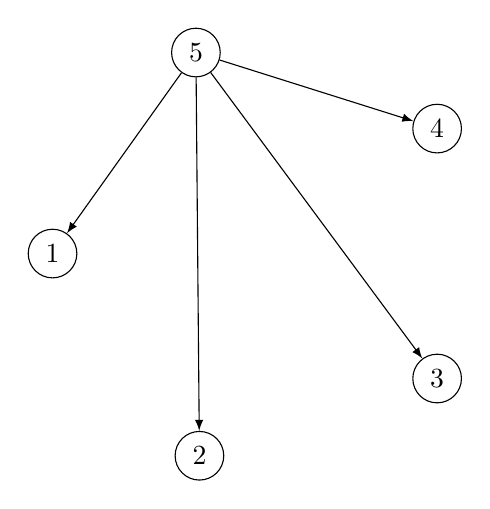
\begin{tikzpicture}[scale=.9]
      \def \n {5}
      \def \ndec {4}
      \def \radius {3cm}
      \def \margin {8} % margin in angles, depends on the radius

      \foreach \s in {1,...,\ndec}
      {
        \node[draw, circle](\s) at ({180 + (360/\n * (\s - 1))}:\radius) {$\s$};
      }
      \node[draw, circle](5) at ({181 + 360/\n * (\n - 1)}:\radius) {$\n$};
      \draw[->, >=latex] (5) -- (1);
      \draw[->, >=latex] (5) -- (2);
      \draw[->, >=latex] (5) -- (3);
      \draw[->, >=latex] (5) -- (4);
    \end{tikzpicture}
    \caption{This diagram demonstrates the downflow of the intermediate keys}
    \label{figures:gka_downflow}
  \end{minipage}
\end{figure}

\subsubsection{Detailed description}
For a more detailed description of the sub-protocol we refer to \cite{mpenc}, however a pseudocode is provided.

Algorithm \ref{upflow_algo} presents an overview of how each upflow message is constructed, using the data received from the previous upflow message.

Algorithm \ref{downflow_algo} presents an overview of how the final, downflow message is constructed using the data received from the last upflow message.

In algorithm \ref{gka_proto_algo} the two previous algorithms (\ref{upflow_algo} and \ref{downflow_algo}) are used in order to execute a complete run of the GKA protocol.
\vfill
\begin{algorithm}[H]
  \KwIn {$\mathcal{P}$ : participants list}
  \KwExtraIn {$\mathcal{S}$ : association table}
  \KwExtraIn {$InterKeys$ : previous intermediate key list}
  \KwExtraIn {$x$ : user's secret key}
  \KwExtraIn {$\hat{Y}$ : the next participant}
  \KwResult{Sends the new intermediate key list to the next participant}
  \Begin
  {
    $inter\_key\_list \leftarrow []$

    $inter\_key\_list.Append(InterKeys.Last() )$

    \ForEach{$k$ in $InterKeys$}
    {
      $inter\_key\_list.Append(k^x)$
    }

    $AuthBroadcast(\hat{Y} \Vert inter\_key\_list, \mathcal{S})$
  }
  \caption{SendUpflow($\mathcal{P}$, $\mathcal{S}$, $InterKeys$, $x$, $\hat{Y}$) --- send the new intermediate key list to the next participant.}
  \label{upflow_algo}
\end{algorithm}
\vfill
\begin{algorithm}[H]
  \KwIn {$\mathcal{P}$ : participants list}
  \KwExtraIn {$\mathcal{S}$ : association table}
  \KwExtraIn {$InterKeys$ : previous intermediate key list}
  \KwExtraIn {$x$ : user's secret key}
  \KwResult{Broadcasts the downflow intermediate key list to the other participants}
  \Begin
  {
    $inter\_key\_list \leftarrow []$

    \ForEach{$k$ in $InterKeys$}
    {
      $inter\_key\_list.Append(k^x)$
	}

    $AuthBroadcast(inter\_key\_list, \mathcal{S})$
  }
  \caption{SendDownflow($\mathcal{P}$, $\mathcal{S}$, $InterKeys$, $x$) --- broadcasts the downflow intermediate key list to the other participants.}
  \label{downflow_algo}
\end{algorithm}
\vfill
\begin{algorithm}[H]
  \KwIn{$sid$ : session ID}
  \KwExtraIn{$\mathcal{S}$ : association table}
  \KwExtraIn{$\mathcal{P}$ : participants list}
  \KwOut{$\mathcal{K}$: the shared secret}
  \Begin
  {
    $x \leftarrow GenerateKey()$

    $\hat{Y}_{prev} \leftarrow \hat{X}.Previous()$

    $\hat{Y}_{next} \leftarrow \hat{X}.Next()$   

    \If{$\hat{Y}_{prev}$ = NULL}{
      $SendUpflow(P, \mathcal{S}, [G], x, \hat{Y}_{next})$
    }
    \Else
    {
      
      \Repeat{$\hat{R} = \hat{X}$}
      {
        $(\hat{Y}, \hat{R} \Vert key\_list) \leftarrow AuthReceive(\mathcal{S})$
      }

      \If{$\hat{Y}$ $\neq$ $\hat{Y}_{prev}$ $\lor$ $\hat{R} \Vert key\_list = \perp$}
      {
        \Return{error}
      }
      \If{$\hat{Y}_{next}$ $\neq$ NULL}
      {
        $SendUpflow(P, \mathcal{S}, key\_list, x, \hat{Y}_{next})$
      }
      \Else
      {
        $final\_key \leftarrow key\_list.Last()$

        $\mathcal{K} \leftarrow final\_key^x$

        $SendDownflow(P, \mathcal{S}, key\_list, x)$

        \Return{$\mathcal{K}$}
      }
    }

    \Repeat{$\hat{Y}$ = $\mathcal{P}.Last()$}
    {
      $(\hat{Y}, key\_list) \leftarrow AuthReceive(\mathcal{S})$
    }
    \If{$key\_list = \perp$}
    {
      \Return{error}
    }
    
    $pos \leftarrow \mathcal{P}.IndexOf(\hat{X})$

    $final\_key \leftarrow key\_list.Reverse().Get(pos)$

    $\mathcal{K} \leftarrow final\_key^x$

	\Return{$\mathcal{K}$}
  }
  \caption{GKA($sid$, $\mathcal{S}$, $\mathcal{P}$) - executes a Group Key Agreement and produces the shared secret in the context of participant $\hat{X}$.}
  \label{gka_proto_algo}
\end{algorithm}

\subsection{Attest}
\label{subsections:attest}
During this sub-protocol the participants must verify that they agree on the $sid$ and the association table $\mathcal{S}$. This is needed for two reasons. First, because $sid$ is required before $\mathcal{S}$ is constructed, and therefore the messages exchanged for the calculation of $sid$ can't be signed. Second, because the participants need to verify that they all have the same view of $\mathcal{S}$.

Each participant calculates the SHA-512 hash of $\mathcal{S}$, which is sorted according to the rule described in \ref{sections:participants_ordering}. Then they broadcast an authenticated message, called "Attest Message", which contains both the $sid$ and the calculated hash. To authenticate the message, each sender signs it using the ephemeral signing key $e_{\hat{X}}$ that has now exchanged with the other participants.

When a participant receives an "Attest Message", first she must verify the signature. Then she must check for two things. First, verify the received hash of $\mathcal{S}$ matches the one she computed herself. Second, check that the received message uses the expected $sid$. A formal description of the Attest sub-protocol in the context of a participant $\hat{X}$ is shown in algorithm \ref{algo:attest}.

Provided that SHA-512 is a cryptographic hash function an attacker can't find two signing keys association tables with the same hash. This means that he is not able to make two participants believe that they have arrived at the same table when they have not. Also by signing the message containing the specific $sid$, a user implicitly verifies that he is using that particular $sid$ for this session.

\begin{algorithm}[H]
  \KwIn{$\mathcal{P}$ : participants list}
  \KwExtraIn{$sid$: the session ID}
  \KwExtraIn{$\mathcal{S}$: the association table}
  \KwOut{$\mathcal{A}$: "OK" if verification went good, "Error" if it went wrong}
  \Begin
  {	
	$M \leftarrow sid \Vert SHA512(\mathcal{S})$
	
	$AuthBroadcast(M)$
	
	$Outstanding \leftarrow \mathcal{P} \textbackslash \{\hat{X}\}$

    \While{$Outstanding \neq \emptyset$}
    {
      $(\hat{Y}, M_{\hat{Y}}) \leftarrow AuthReceive(\mathcal{S})$
      
      \If{$M_{\hat{Y}} = \perp \lor  M_{\hat{Y}} \neq M$}
      {     
        \Return{"Error"}            
        
      }
      \Else{
      
        $Outstanding \leftarrow Outstanding \textbackslash \{\hat{Y}\}$
        
      }
    }

	\Return{"OK"}
  }
  \caption{Attest($\mathcal{P}$, $sid$, $\mathcal{S}$) --- authenticate previously unauthenticated protocol parameters for the current session in the context of participant $\hat{X}$.}
  \label{algo:attest}
\end{algorithm}

\subsection{Communication}
\label{subsections:communication}
Using the Communication sub-protocol, the participants can exchange authenticated and encrypted messages using the association table $\mathcal{S}$ derived from DSKE and the shared key $\mathcal{K}$ derived from GKA.

\subsubsection{Origin authentication}
For origin Authentication we use public key encryption methods. This is done because use of symmetric algorithms would require a participant who wishes to send a message to mac the message $n-1$ times, where $n$ is the number of the participants.

\paragraph{Algorithm}
While describing the DSKE we mentioned that an ephemeral signing key is transmitted by each participant to every other, to be used for message origin verification.

For this purpose we make use of the EdDSA algorithm. This algorithm was selected for its fast key generation, since a new keypair must be generated in each protocol run, and its relatively small signature size.

\paragraph{Signing}
\label{signing}
The signature generation is the last step taken before sending a message. This
way we can sign all the properties of the message to be sent, like the $sid$ or the
recipient (if any). We also avoid any manifestations of the Cryptographic Doom
Principle, which states that if a protocol tries to perform \emph{any}
cryptographic operation before verifying the signature or mac on a received
message, it will somehow fail catastrophically and lead to doom.

Symmetrically the signature verification is the first thing that happens before
any other operation is performed on the received message (cryptographic or not).

\subsubsection{Encryption}

For encryption a shared secret key $\mathcal{K}$ is used by all the members. This is not a problem since the origin authentication is provided by the signatures, and we obviously don't mind any chat member to read a message or we wouldn't participate in the chat in the first place.

To encrypt a message, a user concatenates the shared secret with his personal id and creates a personal key.
This is the actual encryption key.

\[
k_{enc} = H(id_{personal} || master\ key)
\]

For the counter, each user stores locally his personal upper half (8 most significant bytes).
The lower half (8 least significant bytes) are always set to zero.
The top half of the counter is prepended in the sent message.
The ciphertext is produced as follows (where $ctr$ is the top half of the locally stored counter):

\[
ciphertext = AES_{CTR}(k_{enc}, ctr||0, plaintext)
\]

To decrypt a message, a user concatenates the shared secret with the id of the message's sender.
\[
k_{dec} = H(id_{sender} || master\ key)
\]

He uses the prepended top half of the counter.

\[
plaintext = AES_{CTR}(k_{dec}, ctr||0, ciphertext)
\]

This encryption scheme is used, so that the possibility that a certain encryption key and counter pair is eliminated.
If all the participants used the shared secret itself as an encryption key and two users sent a message at the same time, they would use the same counter.
This would be a catastrophic failure.
We discuss why we choose Counter mode in section \ref{setions:Protocol:primitives}

\subsubsection{Transcript}
In order for the shutdown sub-protocol to be executed we need to store the transcript of the chatroom. In reality a seperate transcript is held for the messages from each participant.
The shutdown protocol will then combine all the different transcripts to determine if consensus has been reached.

The transcripts are implemented as linked lists. Each list is kept sorted in lexicographic order.
When a message is to be added in a transcript list, the list is searched linearly to find the position the new message should be placed at.

When user $A$ sends a message, he adds that message to the transcript corresponding to himself.
When he receives a message from user $B$, he adds that message to the transcript corresponding to user $B$.

\subsection{Shutdown}
\label{subsections:shutdown}
During this sub-protocol, the participants end the current session. Chat room transcript consistency is checked and the ephemeral signing keys are published, in order to permit a posteriori modifications of the chat transcript. The revelation of the ephemeral signing keys adds to the protocol's deniability property. However, the protocol is deniable even without publishing the ephemeral signing keys, since the signing keys are deniable in the first place.

For a session to be terminated, a "Shutdown Message" is sent. This message signals to other participants that the shutdown phase should be initiated. It contains the  hash of all the messages sent by the user sending the "Shutdown Message". When a user receives a "Shutdown Message", he also responds with a "Shutdown Message" containing his own messages hash, if he hasn't already sent one.

When one participant has received a "Shutdown Message" from all other participants he can send a "Digest Message". This message contains a digest of all the messages in the chat room and is calculated as follows:
\begin{itemize}
  \item[] Sort the participants using their usernames in lexicographic order.
  \item[] For each participant $i$ (in that order) calculate the hash $h_i = H(S_i)$, where $S_i$ is set of all the messages sent by this user, sorted in lexicographic order too.
  \item[] Calculate the digest $h = H(h_1 || h_2 \dots || h_N)$, where N is the number of participants.
\end{itemize}

When one participant receives a "Digest Message" from some other participant, he checks whether the two of them agree on the chat room transcript. He simply compares the digest he computed locally to the one sent by the other participant. He deduces that consensus is reached only if the two digests are the same.

When one participant has received a "Digest Message" from every other participant, he broadcasts an "End Message". This message signifies that the sender will not use the channel to send any messages anymore.

When a participant receives an "End Message" from all other participants, he is certain that he can release his signing secret key. This is done by broadcasting a message which we shall call "Key Release Message". Now anyone who intercepts the released key can forge chat room messages. However all the participants will no longer accept messages signed with the released secret key, and thus it cannot be used to impersonate its previous owner.

\section{The primitives}
\label{setions:Protocol:primitives}
In the protocol description we talked generally about \dhname Key exchanges, encryption ciphers and signatures.
Here we shall present the specific algorithms and parameters we used in our implementation.

\subsection{Diffie--Hellman Group}
The already existing libotr implementation of the DH key exchange is used.
As a result we use classic Diffie--Hellman , and specifically the group no. 5 \cite{website:dh-rfc} with a 1536 bit modulus.
In the algorithms presented above, all exponentiations are performed in this group.

\subsection{Encryption}

For encryption we use AES-128 in CTR mode, the same cipher as the two-party OTR protocol.

We chose 128-bit AES instead of the 256-bit one because our \dhname group does not provide 256 bit of entropy and evidence suggests that the 128-bit AES key schedule is preferred for security \cite{aes-key-recov} \cite{rijndael-improved-analysis}.

We chose CTR mode because it is malleable.
This increases the deniability properties of the protocol, as described in \cite{otr} and \cite{otr_improvedauth}.

\subsection{Authentication}
For signing we use the EdDSA algorithm over the Ed25519 curve.
This signature scheme was chosen primarily because of its fast key generation.
Each message is signed as a whole.
This means that the signature covers the message and any metadata sent, like session id, counter value etc.

\section{Participants ordering}
\label{sections:participants_ordering}
In many cases, the protocol demands some ordering of the participants. For example, in the Offer step of the Setup phase, the sid contributions should be concatenated in some order before hashing them. Same stands for the public signing keys in the association table, during the Attest step. So we define an ordering rule for the participants, that is used whenever an ordering of elements corresponding to participants is needed.

Given that the application provides the mpOTR protocol with a unique name describing each participant, we make the convention that every ordering of the participants list is made lexicographically based on that unique name. We also define the position of the participant, as his position in this order, starting counting from zero (0).

\section{Identity verification}
The identity of a participant is verified during the DSKE phase.
In order for a participant to be verified the fingerprint of his longterm key must be stored in the known fingerprints file, and be explicitly marked as verified.
In our implementation this file is comma separated and is of the form:

\begin{verbatim}
<account_name>,<protocol>,<buddy_name>,<fingerprint>,<is_verified>
\end{verbatim}

The account name is the "address" of the library user in the form username@host, and is provided by the application.
The protocol is a string that is characteristic of the underlying protocol that the specific account uses.
It is again provided by the application.
The buddy name is the nickname that a user is identified with.
For the time being it is the username part of a users "address".
This implies that the underlying protocol provides addresses which do not change often for a user.
It also means that users from multiple hosts are not allowed or else two users with the same username might conflict.
The above holds for a protocol like jabber for example, but is not the case for protocols like IRC.
As a result our implementation is not fully protocol agnostic at this moment.
Finally the fingerprint is the sha256 hash of the public identity key, and the last field is 1 if the key is verified and 0 otherwise.

This file is read during the plugin start up and initializes the list of all known fingerprints.
When a new chatroom is created, each participant is assigned a list with all known fingerprints used by this participant (from the above list).
When a "Handshake Message" is received the participants known fingerprints list is checked to find (if it exists) a fingerprint matching the currently used public key.
If such a fingerprint is found and it is verified, then the user is verified for this session.
If the found fingerprint is not verified then the participant is not verified.
If no key is found then again the participant is not verified and an entry for this new key is added in the known fingerprints list. 

\section{Handling out-of-order messages}
In the protocol description above, we silently assumed that messages are delivered in-order. In fact, in a distributed context, like the mpOTR, this can be really tricky.

Specificaly in our construction, there are quite a lot messages exchanged during the first four sub-protocols that run automatically to setup the session parameters and hence these messages are usually exchanged in a narrow period of time. Latency differences between participants, either due to the underlying network or due to the participants' equipment may result in out-of-order message delivery to some participants\footnote{In fact, this was one of the first complications we faced during our implementation.}.

For example, there exists a possible scenario where all Offer Messages have been sent, but some of them have only reached some participants in some point of time. In that case, those who have received the Offer Messages proceed to the DSKE sub-protocol and send their Handshake Messages. The latter, may reach participants that haven't yet finished the Offer sub-protocol, and obviously cannot be handled by them.

So, there is a need for some mechanism that ensures that mpOTR messages are handled in-order by the mpOTR Protocol. There are two general approaches to solve this problem in a distributed context.

The first possible approach is the utilization of some synchronization mechanism between the participants so that each participant would ensure that all other participants can handle a message before he sends it. However, this is a rather complicated approach because it would require more messages to be exchanged so that the participants could signal points of synchronization amongst themselves.

We utilized the second approach, which is to make the receivers responsible for handling the received messages in-order. This is a rather simple approach, since it only requires each participant to keep out-of-order messages in a pending queue and handle them when messages supposed to be received ealrier have indeed been received and handled.



\section{Message Structure}
\label{sections:message_structure}

\subsection{Top level encoding}
We follow the OTR rules for the top level encoding of mpOTR messages. That is, all mpOTR messages start with the string "?OTR:" followed by the base64 encoded message and then a "." denoting the end of the message. For a mpOTR message M, we send:

\[ 
  "?OTR:" \Vert Base64(M) \Vert "."
\]

\subsection{Instance tags}
\label{subsections:instance_tags}
Many IM Protocols allow for a client to be logged into the same account from multiple locations and the server may relay messages to all of them. The version 3 of OTR utilizes a distinguishing mechanism, called instance tags.

Instance tags are 32-bit values that are intended to be persistent. If the same client is logged into the same account from multiple locations, the intention is that the client will have different instance tags at each location. All mpOTR messages include the sender's instance tag.

\subsection{Data Types}
We present a list of several data types used in mpOTR messages along with their encoding:
\begin{description}[align=left]
\item [SHORT] Short integers. 2 byte unsigned value, big-endian.
\item [INT] Integers. 4 byte unsigned value, big-endian.
\item [MPI] Multi Precision Integers. 4 byte unsigned len, big-endian. len byte string with each byte of the MPI encoded as 2 hex digits. Negative numbers are prefix with a minus sign and in addition the high bit is always zero to make clear that an explicit sign ist used.
\item [LIST] Lists of any other type. 4 byte unsigned len, big-endian. len encoded list elements.
\item[HASH32] Hashes. 32 bytes of data.
\item[HASH64] Hashes. 64 bytes of data.
\item[CTR] AES CTR-mode counter value. 8 bytes data.
\item[DATA] Opaque variable-length data. 4 byte unsigned len, big-endian. len byte data.
\end{description}

\subsection{Message types}
\label{subsections:message_types}
There are 12 different types of mpOTR messages. Each type is indicated by a positive integer. We have reserved the zero value to indicate non-OTR messages. The list of these types along with the corresponding integer value is shown below:

\hfill
\begin{minipage}{.40\textwidth}
\begin{description}[align=left]
  \item[0] Non-OTR Message
  \item[1] Offer Message
  \item[2] Handshake Message
  \item[3] Confirm Message
  \item[4] Key Message
  \item[5] Upflow Message
  \item[6] Downflow Message
\end{description}
\end{minipage}
\hfill
\begin{minipage}{.40\textwidth}
\begin{description}[align=left]
  \item[7] Attest Message
  \item[8] Data Message
  \item[9] Shutdown Message
  \item[10] Digest Message
  \item[11] End Message
  \item[12] Key Release Message
\end{description}
\end{minipage}
\hfill


\subsection{General message structure}
\begin{figure}[H]
  \begin{bytefield}[bitwidth=0.11111\linewidth]{8}
    \bitheader{0-7} \\
    \begin{rightwordgroup}{Header}
      \bitbox{2}{PV} & \bitbox{2}{MT} & \bitbox{4}{Instance Tag} \\
      \wordbox{4}{Session ID}
    \end{rightwordgroup} \\
    \wordbox{4}{Payload} \\
    \wordbox{2}{Signature}
  \end{bytefield}  
  
  \caption{General message structure}
  \label{figures:general_message_structure}
\end{figure}

In figure \ref{figures:general_message_structure} the general structure of mpOTR messages is shown. Each message contains the following fields:
\begin{itemize}
  \item PV: the Protocol Version. A SHORT indicating the Protocol Version the message is intended for.
  \item MT: the Message Type. A SHORT indicating the type of the message. See \ref{subsections:message_types} for more details.
  \item Instance Tag: an INT indicating the instance tag. See \ref{subsections:instance_tags} for more details.
  \item Session ID: a HASH64 containing the value of $sid$. Not existent in Offer Messages.
  \item Payload: specific data dependent for each type of message. See \ref{subsections:payload_structures} for more details.
  \item Signature: the signature covering all data above, used to authenticate the message. Not existent in all message types.
\end{itemize}

There are only a few exceptions. Offer Messages contain no Session ID in the header, since $sid$ has not been established yet. Offer and DAKE Messages contain no Signature since the association table $\mathcal{S}$ has not been constructed yet. Shutdown KeyRelease Messages also contain no Signature since authentication is not required.

\subsection{Payload structures}
\label{subsections:payload_structures}
In the following paragraphs we show the payload structure of each mpOTR message type. We also briefly describe each field.

\subsubsection{Offer Message Payload}
\begin{figure}[H]
  \begin{bytefield}[bitwidth=0.11111\linewidth]{8}
    \bitheader{0-7} \\
    \bitbox{4}{Position} & \bitbox[lrt]{4}{} \\
    \wordbox[lr]{1}{SID Contribution} \\
    \bitbox[l]{4}{} & \bitbox[rb]{4}{} \\
    \bitbox[lrb]{4}{}
  \end{bytefield}
  \caption{The structure of Offer Message payload}
\end{figure}

\begin{itemize}
  \item Position: an INT indicating the sender's position in the ordered list of the participants.
  \item SID Contribution: a HASH32 containing the sender's contribution for the construction of the $sid$.
\end{itemize}

\subsubsection{Handshake Message Payload}
\begin{figure}[H]
  \begin{bytefield}[bitwidth=0.11111\linewidth]{8}
    \bitheader{0-7} \\
    \wordbox[lrt]{1}{Ephemeral PubKey} \\
    \wordbox[blr]{1}{$\cdots$} \\
    \wordbox[lrt]{1}{Longterm PubKey} \\
    \wordbox[blr]{1}{$\cdots$}
  \end{bytefield}
  \caption{The structure of Handshake Message payload}
\end{figure}

\begin{itemize}
  \item Ephemeral PubKey: a MPI containing the public part of the ephemeral key.
  \item Longterm PubKey: a MPI containing the public part of the longterm key.
\end{itemize}

\subsubsection{Confirm Message Payload}
\begin{figure}[H]
  \begin{bytefield}[bitwidth=0.11111\linewidth]{8}
    \bitheader{0-7} \\
    \bitbox{4}{Recipient} & \bitbox[tlr]{4}{} \\
    \wordbox[lr]{1}{TDH MAC} \\
    \bitbox[l]{4}{} & \bitbox[rb]{4}{} \\
    \bitbox[lrb]{4}{}
  \end{bytefield}
  \caption{The structure of Confirm Message payload}
\end{figure}

\begin{itemize}
  \item Recipient: an INT indicating the participant this message is intended for. It's actually his position in the ordered participants list.
  \item TDH MAC: a Triple Diffie-Hellman MAC. A HASH32 containing the MAC value for a magic number.
\end{itemize}

\subsubsection{Key Message Payload}
\begin{figure}[H]
  \begin{bytefield}[bitwidth=0.11111\linewidth]{8}
    \bitheader{0-7} \\
    \bitbox{4}{Recipient} & \bitbox[tlr]{4}{} \\
    \wordbox[lr]{1}{TDH MAC} \\
    \bitbox[l]{4}{} & \bitbox[rb]{4}{} \\
    \bitbox[lrb]{4}{} & \bitbox[tlr]{4}{} \\
    \wordbox[lr]{1}{Key} \\
    \wordbox[blr]{1}{$\cdots$} \\
  \end{bytefield}
  \caption{The structure of Key Message payload}
\end{figure}

\begin{itemize}
  \item Recipient: an INT indicating the participant this message is intended for. It's actually his position in the ordered participants list.
  \item TDH MAC: a Triple Diffie-Hellman MAC. A HASH32 containing the MAC value for the following key.
  \item Key: DATA containing the encrypted public part of the ephemeral signing key.
\end{itemize}

\subsubsection{Upflow Message Payload}
\begin{figure}[H]
  \begin{bytefield}[bitwidth=0.11111\linewidth]{8}
    \bitheader{0-7} \\
    \bitbox{4}{Recipient} & \bitbox{4}{ListLen} \\
    \begin{rightwordgroup}{\parbox{4em}{\raggedright ListLen number of list elements}}
      \wordbox[lrt]{1}{1st Key} \\
      \wordbox[blr]{1}{$\cdots$} \\
      \wordbox[lrt]{1}{2nd Key} \\
      \wordbox[blr]{1}{$\cdots$} \\
      \wordbox[blr]{2}{$\cdots$} \\
      \wordbox[lrt]{1}{n-th Key} \\
      \wordbox[blr]{1}{$\cdots$}
    \end{rightwordgroup}
  \end{bytefield}
  \caption{The structure of Upflow Message payload}
\end{figure}

\begin{itemize}
  \item Recipient: an INT indicating the participant this message is intended for. It's actually his position in the ordered participants list.
  \item ListLen: an INT containing the length of the following key list.
  \item i-th Key: an MPI containing the i-th key of the intermediate key list.
\end{itemize}

\subsubsection{Downflow Message Payload}
\begin{figure}[H]
  \begin{bytefield}[bitwidth=0.11111\linewidth]{8}
    \bitheader{0-7} \\
    \begin{rightwordgroup}{\parbox{4em}{\raggedright ListLen number of list elements}}
      \bitbox{4}{ListLen} & \bitbox[tlr]{4}{} \\
      \wordbox[lr]{1}{1st Key} \\
      \wordbox[blr]{1}{$\cdots$} \\
      \wordbox[lrt]{1}{2nd Key} \\
      \wordbox[blr]{1}{$\cdots$} \\
      \wordbox[blr]{2}{$\cdots$} \\
      \wordbox[lrt]{1}{n-th Key} \\
      \wordbox[blr]{1}{$\cdots$}
    \end{rightwordgroup}
  \end{bytefield}
  \caption{The structure of Downflow Message payload}
\end{figure}

\begin{itemize}
  \item ListLen: an INT containing the length of the following key list.
  \item i-th Key: an MPI containing the i-th key of the intermediate key list.
\end{itemize}

\subsubsection{Attest Message Payload}
\begin{figure}[H]
  \begin{bytefield}[bitwidth=0.11111\linewidth]{8}
    \bitheader{0-7} \\
    \wordbox{2}{Session ID} \\
    \wordbox{2}{Association Table Hash} 
  \end{bytefield}
  \caption{The structure of Attest Message payload}
\end{figure}

\begin{itemize}
  \item Session ID: a HASH64 containing the value of $sid$.
  \item Association Table Hash: a HASH64 containing the hash of the association table $\mathcal{S}$.
\end{itemize}

\subsubsection{Data Message Payload}
\begin{figure}[H]
  \begin{bytefield}[bitwidth=0.11111\linewidth]{8}
    \bitheader{0-7} \\
    \wordbox{1}{CTR} \\
    \wordbox[tlr]{1}{Ciphertext} \\
    \wordbox[blr]{1}{$\cdots$} \\
  \end{bytefield}
  \caption{The structure of Data Message payload}
\end{figure}

\begin{itemize}
  \item CTR: a CTR containing the top half of the counter for AES CTR-mode.
  \item Ciphertext: a DATA containing the encrypted message.
\end{itemize}

\subsubsection{Shutdown Message Payload}
\begin{figure}[H]
  \begin{bytefield}[bitwidth=0.11111\linewidth]{8}
    \bitheader{0-7} \\
    \wordbox{2}{Shutdown Hash} \\
  \end{bytefield}
  \caption{The structure of Shutdown Message payload}
\end{figure}

\begin{itemize}
  \item Shutdown Hash: a HASH64 containing the hash of the sender's transcript.
\end{itemize}

\subsubsection{Digest Message Payload}
\begin{figure}[H]
  \begin{bytefield}[bitwidth=0.11111\linewidth]{8}
    \bitheader{0-7} \\
    \wordbox{2}{Digest} \\
  \end{bytefield}
  \caption{The structure of Digest Message payload}
\end{figure}

\begin{itemize}
  \item Digest: a HASH64 containing the hash of all transcripts.
\end{itemize}

\subsubsection{End Message Payload}
End Messages contain no payload.

\subsubsection{Key Release Message Payload}
\begin{figure}[H]
  \begin{bytefield}[bitwidth=0.11111\linewidth]{8}
    \bitheader{0-7} \\
    \wordbox[tlr]{1}{Key} \\
    \wordbox[blr]{1}{$\cdots$} \\
  \end{bytefield}
  \caption{The structure of Key Release Message payload}
\end{figure}

\begin{itemize}
  \item Key: a DATA containing the value of the key to be revealed.
\end{itemize}